\documentclass[a4paper, 12pt, twoside]{article}
\usepackage[outer={2.5cm},inner={4cm},tmargin={2.5cm},bmargin={2cm}]{geometry}
\usepackage{amsmath}
\usepackage{amssymb}
\usepackage{amsthm}
\usepackage{babel}[english]
\usepackage{hyperref}
\usepackage{colonequals}
\usepackage{xfrac}
\usepackage{tikz}
\usepackage{tikz-cd}

\usepackage{graphicx}
\usepackage{caption}

\setlength{\parindent}{0mm}
\setcounter{MaxMatrixCols}{100}

\newcommand{\R}[0]{\mathbb{R}}
\newcommand{\N}[0]{\mathbb{N}}
\newcommand{\T}[0]{\mathcal{T}}
\newcommand{\NB}[0]{\mathcal{N}}
\newcommand{\PowS}[0]{\mathfrak{P}}
\newcommand*{\logeq}{\ratio\Leftrightarrow}
\newcommand*{\longeq}{\ratio\Longleftrightarrow}
\newcommand*{\bigdot}{\mathpalette\bigcdot@{.5}}
\newcommand{\sd}{{\rm sd}}
  
\title{Masters thesis\\Title}
\author{Yannik Höll}
\date{\today}

\newtheoremstyle{break}%
{7pt}{7pt}%
{}{}%
{\bfseries}{:}% % Note that final punctuation is omitted.
{\newline}{}

\theoremstyle{break}
\newtheorem{thm}{Theorem}[section]

\theoremstyle{break}
\newtheorem{rem}[thm]{Remark}
\newtheorem{lemma}[thm]{Lemma}
\newtheorem{defin/}[thm]{Definition}
\newtheorem{col}[thm]{Corollary}
\newtheorem{ex}[thm]{Example}

\newenvironment{defin}
    {\renewcommand{\qedsymbol}{$\spadesuit$}\pushQED{\qed}\begin{defin/}}
    {\popQED\end{defin/}}

% for centering the title page
\usepackage{titling}

% TODO: add a ending mark (solid black square) as the end of definitions

\linespread{1.5}
\begin{document}

\begin{titlingpage}
    \maketitle
\end{titlingpage}
\clearpage

\tableofcontents
\pagebreak

\clearpage

\nocite{*}


\section*{Abstract}
\section{Introduction}
\section{Topology, Topological Algebra and Algebraic Topology}

\section{Simplicial Homology}

\subsection{Abstract simplicial complexes}

\begin{defin}
    Let $X$ be a non-empty set. Then a collection $\mathcal{K} \subseteq \PowSF(X)$ of finite subsets of $X$ is called a 
    \textbf{simplicial complex} of $X$ if
    \begin{itemize}
        \item $\bigcup \mathcal{K} = X$,
        \item $\forall \sigma\in\mathcal{K} \colon \tau \subseteq \sigma \; \Rightarrow \; \tau \in \mathcal{K}$.
    \end{itemize}
    The elements of the set $V(\mathcal{K}) := \bigcup \mathcal{K}$ are the \textbf{vertecies} of $\mathcal{K}$ and
    elements of $\mathcal{K}$ itself are the \textbf{simplicies}. Given a simplex $\sigma \in \mathcal{K}$ then the sets
    $\; \sigma \setminus \{x\} \;$ for $x \in \sigma$ are called the \textbf{faces} of $\sigma$.

    Let $\sigma \in \mathcal{K}$ then $\dim \sigma = |\sigma| -1$ is the \textbf{dimension} of $\sigma$. The dimension of $\mathcal{K}$ is
    \begin{equation*}
      \dim \mathcal{K} = \max\{\dim \sigma\colon \sigma \in \mathcal{K}\}.
    \end{equation*} 
    
    Let $Y$ be another non-empty set and $\mathcal{L}$ be a simplicial complex on $Y$. A map $f: V(\mathcal{K}) \to V(\mathcal{L})$ is called 
    a \textbf{simplicial} map if
    \begin{equation*}
        \forall \sigma \in \mathcal{K}\colon f(\sigma) \in \mathcal{L}.
    \end{equation*}
    If $f$ is bijective and $f^{-1}\colon \mathcal{L} \to \mathcal{K}$ is a simplicial map then $f$ is an \textbf{combinatorial isomorphism}.
    If $\iota\colon \mathcal{L} \to \mathcal{K}$ is an inclusion, we say that $\mathcal{L}$ is a \textbf{subcomplex} of $\mathcal{K}$ if $\iota$ is a simplicial map.
\end{defin}

% Simple Example of a simplicial complex
\begin{ex}\label{ex:seqcom}
  Let $n \in \N^+$ then $\mathcal{K}_n$ defined as
  \begin{equation*}
    \mathcal{K}_n = \PowS([n])
  \end{equation*}
  is a sequence of simplicial complexes. For example $\mathcal{K}_2 := \{\emptyset, \{0\}, \{1\}, \{0,1\}\}$.
\end{ex}

\begin{defin}
    Let $X$ be a set, $H$ be a group and $\mathcal{K}$ be a simplicial complex on $X$. If there is an 
    group action $\lambda \colon H \times X \to X$ of $H$ on $X$ then
    the complex $\mathcal{K}$ is an \textbf{$H$-complex} if the map
    \begin{equation*}
        \lambda_h \colon \mathcal{K} \to \mathcal{K}, \: \sigma \mapsto \{ \lambda(h, \tau)\colon \tau \in \sigma \}
    \end{equation*}
    is a simplicial map for all $h \in H$.
\end{defin}

\begin{defin}
    A poset (partially ordered set) is a pair $(P, \preceq)$ where 
    $P$ is a non-empty set and 
    $\preceq$ is a binary relation on $P$ which has the following properties:
    \begin{enumerate}
        \item \textit{Reflexivity}: $\forall x \in P\colon x \preceq x$,
        \item \textit{Antisymmetry}: $\forall x, y \in P\colon (x \preceq y \: \land \: y \preceq x) \Rightarrow (x = y)$,
        \item \textit{Transitivity}: $\forall x, y, z \in P\colon (x \preceq y \: \land \: y \preceq z) \Rightarrow (x \preceq z)$.
    \end{enumerate}
    A chain in $P$ is a subset $C \subseteq P$ which is totally ordered, i.e.
    \begin{equation*}
        \forall x, y \in C\colon x \preceq y \: \lor \: y \preceq x.
    \end{equation*}
\end{defin}

\begin{ex}
    If $X$ is a non-empty set then the pair $(\PowS(X), \subseteq)$ forms a poset.
\end{ex}

The last example establishes the following definition:
If $X$ is a non-empty family of sets then $P(X) := (X, \subseteq)$ is the poset generated by $X$. The elements of $X$
are the elements of the poset and the binary relation of set inclusion is the partial order.

\begin{defin}
    Let $\mathcal{K}$ be an abstract simplicial complex. The \textbf{barycentric subdivision} $\sd(\mathcal{K})$ of $\mathcal{K}$
    is the abstract simplicial complex with $\mathcal{K}$ as the set of vertecies and all chains in $P(\mathcal{K})$ as simplicies.
\end{defin}

\begin{thm}
    If $\mathcal{K}$ is a abstract simplicial complex, then $\sd(\mathcal{K})$ is a well-defined abstract simplicial complex.
\end{thm}

\begin{proof}
    Let $\sigma \in \sd(\mathcal{K})$. Now let $\tau \subseteq \sigma$. Since $\sigma$ was totally ordered $\tau$ is also totally ordered.
    This means that $\tau \in \mathcal{K}$.
\end{proof}

We need a way to turn an abstract simplicial complex into a geometric structure such that it can be analyzed with the tools provided by algebraic topology. This means that there should be a map from the simplicies of the abstract complex to $n$-dimensional euclidian space. This map is called the \textbf{geometric realization} of the abstract simplicial complex which maps it to a geometric simplicial complex. 
These geometric complexes consist of polyhedra. They are constructed by "gluing" 
together points, straight line segments, polyhedra and their higher dimensional generalizations.
It will be clear that these two types of objects internally encode the same combinatorical structure. 

\begin{defin}
    Let $n,k \in \N$ and let $x_0, x_1, \ldots, x_k \in \R^n$. 
    The vectors are called \textbf{affinely independent} if
    \begin{equation*}
        \sum\limits_{i=0}^k \alpha_i = 0 \; \land \; \sum\limits_{i=0}^k \alpha_i x_i = 0 \; \Rightarrow \; \alpha_0 = \alpha_1 = \ldots = \alpha_k = 0, 
    \end{equation*} with $\alpha_j \in \R$ and $j = 0, 1, \ldots, k$.
\end{defin}

\begin{defin}
    Let $n,k \in \N$ and let $x_0, x_1, \ldots, x_k \in \R^n$. The convex hull of the vectors $x_i$ is
    \begin{equation*}
        {\rm co} (A) = {\rm co}(x_0, x_1, \ldots, x_k) := \{ t_0 x_0 + t_1 x_1 + \cdots + t_k x_k \colon t_i \in [0, 1], \sum\limits_{i=0}^k t_i = 1\}
    \end{equation*}
    where $A = \{x_i\colon i \in [k]\}$.  
\end{defin}

\begin{rem}
  Let $d\in\N$ and $A,B \subseteq \R^d$. If $A \cup B$ affinely independent, then
  \begin{equation*}
    ({\rm co} A) \cap ({\rm co}B) = {\rm co}(A \cap B).
  \end{equation*}
\end{rem}

\begin{proof}
  The inclusion ${\rm co}(A\cap B) \subseteq {\rm co}A \cap {\rm co}B$ is trivial.

  For the other inclusion take $x \in {\rm co}(A) \cap {\rm co}(B)$. This means that there exist to representations of $x$ of the form
  \begin{align*}
    x = \sum\limits_{i=1}^m\alpha_i a_i, \\
    x = \sum\limits_{j=1}^n\beta_j b_j,
  \end{align*}
  for $m,n \in \N$, $a_i \in A$ for all $i = 1, \ldots, m$ with $\sum\limits_{i=1}^m \alpha_i = 1$ and $b_j \in B$ for all $j =1, \ldots,n$ with $\sum\limits_{j=1}^n\beta_j = 1$.
  Now subtract both representations of $x$. It follows that
  \begin{equation*}
    \sum\limits_{i=1}^m\alpha_i a_i - \sum\limits_{j=1}^n\beta_j b_j = 0 \: \land \: \sum\limits_{i=1}^m \alpha_i - \sum\limits_{j=1}^n\beta_j = 0.
  \end{equation*}
  Since $A \cup B$ are affinely indepent this means that either all coefficients are zero or there exist indicies for which $a_i = b_j$. Since the sum of the coefficients $a_i$ and $b_j$ sum up to one the case that all coefficients are zero is not possible and thus we have that both convex combinations of $x$ can only contain points which lie in $A \cap B$. So $x \in {\rm co}(A\cap B)$.
\end{proof}

Affine independence of the vectors makes sure that the convex hull of vectors is not degenerated.
For example it is expected that the convex hull of three vectors in $\R^2$ is a triangle. But in the degenerate case that the points are all the same
or the points lie in a straight line, this is not true. When it is assumed that the points are affinely independent, these cases are excluded. 

\begin{defin}
  A \textbf{geometric realization} of an abstract simplicial complex $\mathcal{K}$ is a map
  \begin{equation*}
    f\colon V(\mathcal{K}) \to \R^d
  \end{equation*}

  with $d \in \N$ such that
  \begin{enumerate}
    \item $\forall \sigma \in \mathcal{K}\colon f(\sigma)$ affinely independent,
    \item $\forall \sigma_1, \sigma_2\in \mathcal{K}\colon ({\rm co}f(\sigma_1)) \cap ({\rm co} f(\sigma_2)) = {\rm co}f(\sigma_1 \cap \sigma_2)$.
  \end{enumerate}
    Given a geometric realization $f$ for $\mathcal{K}$, then $\lVert K \rVert_f = f(\mathcal{K})$. The symbol $\lVert \mathcal{K} \rVert$ refers the an arbitrary geometric realization of $\mathcal{K}$ in the smallest dimension $d$ that is possible.
    Let $x \in \lVert K \rVert_f$. Then $x$ is in ${\rm co}A_x$ for exactly one set $\{f(v_1), f(v_2), \ldots, f(v_k)\} = A_x \subseteq f(V(\mathcal{K}))$ for which the following equations hold 
    \begin{equation*}
      x = \sum\limits_{i=1}^k t_i \cdot f(v_i), \hspace*{30px} \sum\limits_{i=1}^k t_i = 1, 
    \end{equation*}
    where $k\in \N^+$ and $t_i \in [0, 1]$ for all $i \in \{1, 2, \ldots, k\}$. Define $\alpha_v(x)$ as
    \begin{equation*}
      \alpha_v(x) = \begin{cases}
        &t_i, \: v \in A_x, \\
        &0, \: \text{otherwise}
      \end{cases}
    \end{equation*}
    for $v \in V(\mathcal{K})$.
    The $\alpha_v(x)$ are which are non-zero are called the \textbf{barycentric coordinates} of $x$.
\end{defin} 

To show that $\lVert \mathcal{K} \rVert$ for an abrbitrary simplicial complex is well-defined, we need the following theorem.

\begin{thm}
  Let $\mathcal{K}$ be a simplicial complex with $\dim \mathcal{K} = n \in \N$. Then there exists a geometric realization $f\colon V(\mathcal{K}) \to \R^{2d+1}$.
\end{thm}

\begin{proof}
  This is a direct consequence of \cite[Lemma 5.1.1]{using2003}.
\end{proof}

\begin{lemma}\label{lem:sdsimeq}
  Let $\mathcal{K}$ be a simplicial complex. Then \[\lVert \mathcal{K} \rVert \simeq \lVert \sd(\mathcal{K}) \rVert.\]
\end{lemma}

\begin{proof}
  See \cite[p. 84]{MunAlTop}.
\end{proof}

\begin{figure}[ht!]
    \centering
    \begin{tikzpicture}[scale=1.7]
\node[fill=black, circle, inner sep=2pt, label=below:{$0$}] (A) at (0,0) {};
\node[fill=black, circle, inner sep=2pt, label=below:{$2$}] (B) at (2,0) {};
\node[fill=black, circle, inner sep=2pt, label=above:{$1$}] (C) at (1,2) {};
\node[align=center] at (1,-0.5) (label1) {$\mathcal{K}$};

\node[fill=black, circle, inner sep=2pt, label=below:{$0$}] (D) at (6,0) {};
\node[fill=black, circle, inner sep=2pt, label=below:{$2$}] (E) at (8,0) {};
\node[fill=black, circle, inner sep=2pt, label=above:{$1$}] (F) at (7,2) {};
\node[fill=black, circle, inner sep=2pt, label=above:{$01$}] (G) at (6.5,1) {};
\node[fill=black, circle, inner sep=2pt, label=above:{$12$}] (H) at (7.5,1) {};
\node[fill=black, circle, inner sep=2pt, label=below:{$02$}] (I) at (7,0) {};
\node[fill=black, circle, inner sep=2pt] (J) at (7,2/3) {}; 
\node[align=center] at (7,-0.5) (label1) {$\sd(\mathcal{K})$};

\node at (3, 1) (AS) {};
\node at (5, 1) (AE) {};

\draw (A) -- (B);
\draw (B) -- (C);
\draw (C) -- (A);


\draw (D) -- (E);
\draw (D) -- (F);
\draw (F) -- (E);
\draw (C) -- (A);
\draw (D) -- (J);
\draw (E) -- (J);
\draw (F) -- (J);
\draw (H) -- (J);
\draw (I) -- (J);
\draw (G) -- (J);

\node[fill=white, inner sep=1.5pt] at (6.5,1.25) {$01$};
\node[fill=white, inner sep=1.5pt] at (7.5,1.25) {$12$};
\node[fill=white, inner sep=1.5pt] at (7,-0.25) {$02$};
\node[fill=white, inner sep=1.1pt] at (7,1) {$123$};
\draw [|->, thick] (AS) -- node[above] {$\sd$} (AE);
    \end{tikzpicture} 
  \caption{Barycentric subdivision of the 2-dimensional simplex.}
\end{figure}


\begin{defin}
  Let $d \in \N^d$ and let $f\colon V(\mathcal{K}) \to \R^d$. The \textbf{affine extension} $\lVert f \rVert$ of this function is defined as
  \begin{equation*}
    \lVert f \rVert\colon \lVert \mathcal{K} \rVert \to \R^d,\: x \mapsto \sum\limits_{v \in V(\mathcal{K})} \alpha_v(x) f(v).
  \end{equation*}
\end{defin}

\begin{ex}
  Take the sequence of simplicial complexes $\mathcal{K}_n$ from Example \ref{ex:seqcom}. A possible geometric realization of these complexes is
  \begin{equation*}
    f_n\colon V(\mathcal{K}_n) \to \R^n, k \mapsto e_k 
  \end{equation*}
  where $e_k$ for $k \in [n]$ is the $k$-th canonical basis vector of $\R^n$. This sequence of complexes have the property that there is a homeomorphism $\psi\colon \lVert \mathcal{K}_n \rVert_f \to \mathbb{S}^{n-1}$.
\end{ex}

\begin{defin}
  Let $\mathcal{K}$ and $\mathcal{L}$ be abstract simplicial complexes. The \textbf{join} of these complexes is defined as
  \begin{equation*}
    \mathcal{K} \star \mathcal{L} := \{\sigma \sqcup \tau\colon \sigma \in \mathcal{K}, \tau \in \mathcal{L} \}.
  \end{equation*}
  The $n$-fold join $\bigstar_{i \in [n]} \mathcal{K}_i$ is defined by
  \begin{equation*}
    \bigstar_{i=0}^{n-1} \mathcal{K}_i = \bigstar_{i \in [n]} K_i := \{\sigma_0 \sqcup \cdots \sqcup \sigma_{n-1}\colon \forall i\in [n]\colon \sigma_i \in \mathcal{K}_i\}.
  \end{equation*}
  Since the disjoint union is associative up to an isomorphism, this operation is well-defined.
  The special case ${\rm Cone}(\mathcal{K}) = \mathcal{K} \star \PowS_{\leq 1}(\{ \Delta \})$ is the cone of $\mathcal{K}$ with a cone point $\Delta$. Given a finite subsequence of simplical subcomplexes $(L_i)_{i\in [n]}$ of $\mathcal{K}$ define \[{\rm Cone}(\mathcal{K}, (L_i)_{i\in [n]}) := \mathcal{K} \cup {\rm Cone}(L_1) \cup \cdots \cup {\rm Cone}(L_{n-1})\] for $n \in \N$. The cone points are distinct for each cone.

  
  Now define basepoints $v_k \in V(\mathcal{K}), v_l \in V(\mathcal{L})$ of the two simplicial complexes. The \textbf{wedge} of $\mathcal{K}$ with $\mathcal{L}$ is defined as
  \begin{equation*}
    \mathcal{K} \lor \mathcal{L} := \: \faktor{\mathcal{K} \sqcup \mathcal{L}}{\sim}
  \end{equation*}
  where $\sim$ is the equivalence relation, that identifies the basepoints.
  The $n$-fold wedge $\bigvee_{i=0}^{n-1} \mathcal{K}_i= \bigvee\limits_{i \in [n]} \mathcal{K}_i$ for simplicial complexes $\mathcal{K}$ is the $n$-fold disjoint union with the same equivalence relation.
\end{defin}

\begin{ex}
  Let $\mathcal{K} = \mathcal{L}$ with $V(\mathcal{K}) = [3]$ be the two-dimensional simplex (a triangle in the plain) and choose the basepoints $1 \in V(\mathcal{K}), 1 \in V(\mathcal{L})$. Then a geometric realization of the wedge $\mathcal{K} \lor \mathcal{L}$ is depicted in the Figure \ref{fig:simwejo}.
  \begin{figure}[h!]
    \centering
    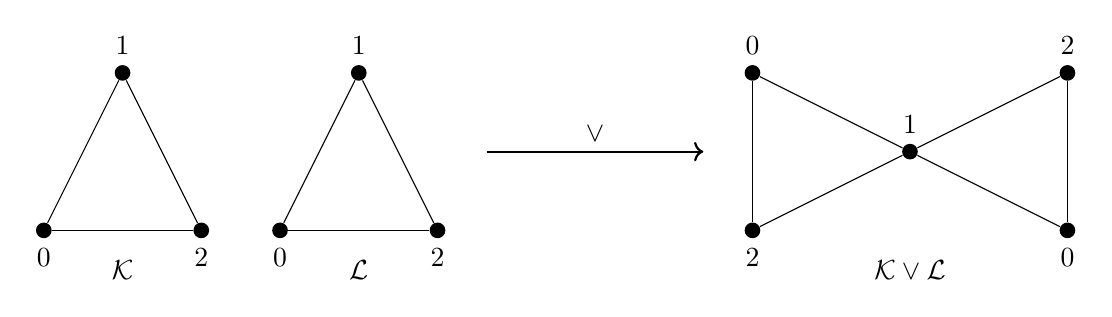
\begin{tikzpicture}
\node[fill=black, circle, inner sep=2pt, label=below:{$0$}] (A) at (0,0) {};
\node[fill=black, circle, inner sep=2pt, label=below:{$2$}] (B) at (2,0) {};
\node[fill=black, circle, inner sep=2pt, label=above:{$1$}] (C) at (1,2) {};
\node[align=center] at (1,-0.5) (label1) {$\mathcal{K}$};

\node[fill=black, circle, inner sep=2pt, label=below:{$0$}] (D) at (3,0) {};
\node[fill=black, circle, inner sep=2pt, label=below:{$2$}] (E) at (5,0) {};
\node[fill=black, circle, inner sep=2pt, label=above:{$1$}] (F) at (4,2) {};
\node[align=center] at (4,-0.5) (label2) {$\mathcal{L}$};

\node[fill=black, circle, inner sep=2pt, label=above:{$0$}] (G) at (9,2) {};
\node[fill=black, circle, inner sep=2pt, label=below:{$2$}] (H) at (9,0) {};
\node[fill=black, circle, inner sep=2pt, label=above:{$1$}] (I) at (11,1) {};
\node[fill=black, circle, inner sep=2pt, label=above:{$2$}] (J) at (13,2) {};
\node[fill=black, circle, inner sep=2pt, label=below:{$0$}] (K) at (13,0) {};
\node[align=center] at (11,-0.5) (label3) {$\mathcal{K} \lor \mathcal{L}$};

\node at (5.5, 1) (AS) {};
\node at (8.5, 1) (AE) {};

\draw (A) -- (B);
\draw (B) -- (C);
\draw (C) -- (A);

\draw (D) -- (E);
\draw (D) -- (F);
\draw (E) -- (F);

\draw (G) -- (I);
\draw (G) -- (H);
\draw (H) -- (I);
\draw (J) -- (K);
\draw (J) -- (I);
\draw (K) -- (I);

\draw [->, thick] (AS) -- node[above] {$\lor$} (AE);
    \end{tikzpicture} 
    \caption{Examples of the wedge of simplicial complexes.}\label{fig:simwejo}
\end{figure}

\begin{lemma}\label{lem:seqhom}
  Let $\mathcal{K}$ be a simplicial complex and let $(L_i)_{i\in [p]}$ be a sequence of subcomplexes of $\mathcal{K}$ for $p \in \N$. If $L_i$ is empty or contractible for each $i \in [p]$ then \[\lVert {\rm Cone}(\mathcal{K}, (L_i)_{i\in [p]}) \rVert \simeq \lVert \mathcal{K} \rVert.\]
\end{lemma}

\begin{proof}
  We know that each ${\rm Cone}(L_i)$ for $i \in [p]$ is contratible. So there is a homotopy equivalence to a one point space. Choose a point in $\lVert \mathcal{K} \rVert$ to which ${\rm Cone}(L_i)$ is contracted to for each $L_i$. The we start with $i = 1$ and can define a homotopy equivalence that keeps $\mathcal{K}$ fixed and contracts the cone over $L_i$ to the chosen point in $\mathcal{K}$. This shows that $\lVert \mathcal{K} \cup {\rm Cone}(L_0) \rVert \simeq \lVert \mathcal{K} \rVert$. The statement follows by induction on $i$. 
\end{proof}

Now consider the complexes $\mathcal{K} = \PowS_{\leq 1}(\{0, 1\})$ and $\mathcal{L} = \PowS_{\leq 1}(\{2, 3\})$. The geometric realization of the join $\mathcal{K} \star \mathcal{L}$ of these complexes can be seen in Figure \ref{fig:simjo}. From the figure it becomese apperent that $\lVert \mathcal{K} \star \mathcal{L} \rVert$ is homeomorphic to $\mathbb{S}^1$.

  \begin{figure}[h!]
  \centering
  \begin{tikzpicture}
\node[fill=black, circle, inner sep=2pt, label=below:{$0$}] (D) at (1,0) {};
\node[fill=black, circle, inner sep=2pt, label=below:{$1$}] (E) at (2,0) {};
\node[align=center] at (1.5,-1) (label3) {$\mathcal{K}$};

\node[fill=black, circle, inner sep=2pt, label=below:{$2$}] (D) at (2,2) {};
\node[fill=black, circle, inner sep=2pt, label=below:{$3$}] (E) at (3,2) {};
\node[align=center] at (2.5,1) (label3) {$\mathcal{L}$};

\node[fill=black, circle, inner sep=2pt, label=above:{$0$}] (G) at (7,2) {};
\node[fill=black, circle, inner sep=2pt, label=below:{$3$}] (H) at (7,0) {};
\node[fill=black, circle, inner sep=2pt, label=above:{$2$}] (I) at (9,2) {};
\node[fill=black, circle, inner sep=2pt, label=below:{$1$}] (K) at (9,0) {};
\node[align=center] at (8,-0.5) (label3) {$\mathcal{K} \star \mathcal{L}$};

\node at (4, 1) (AS) {};
\node at (6, 1) (AE) {};

\draw (G) -- (H);
\draw (H) -- (K);
\draw (K) -- (I);
\draw (I) -- (G);

\draw [->, thick] (AS) -- node[above] {$\star$} (AE);
  \end{tikzpicture}
  \caption{Example of the join of simplicial complexes.}\label{fig:simjo}
  \end{figure}
\end{ex}

The fact that the join of a two points with two points results in a simplicial complex that has a geometric realization that is homeomorphic does not only work with $\mathbb{S}^1$. This fact holds more generally for the n-fold join of 2-point simplicial complexes. 

\begin{lemma}\label{lem:simexkn}
  Let $\mathcal{K}_n := \PowS_{\leq 1}(\{(-1, n), (1, n)\})$ for $n \in \N^+$, then
  \begin{equation*}
    \left\lVert \bigstar_{i=1}^k \mathcal{K}_i \right\rVert \: \cong \: \mathbb{S}^{k-1}.
  \end{equation*}
\end{lemma}

\begin{proof}
  A geometric realization of this complex is as follows
  \begin{equation*}
    f\colon V(\bigstar_{i=1}^k \mathcal{K}_i) \to \R^n, \: (x, i) \mapsto x \cdot e_i
  \end{equation*}
  which means that the vertecies get mapped to the canonical basis vectors of $\R^n$ and their negations. 
  This geometric realization forms the boundary of the $n$-crosspolytope\footnote{This $n$-crosspolytope is $\{(x_1, \ldots, x_n) \in \R^n\colon |x_1| + \cdots + |x_n| \leq 1 \}$. The boundary $\partial P^n$ of the polytope is formed by all points with $1$-norm equal to $1$.} for each $n \in \N^+$. It is homeomorphic to the sphere by the homeomorphism
  \begin{equation*}
    \varphi\colon \mathbb{S}^n \to \partial P^n, \: x \mapsto \lVert x \rVert_1^{-1} \cdot x. 
  \end{equation*}
\end{proof}

\begin{figure}[ht!]
  \centering
  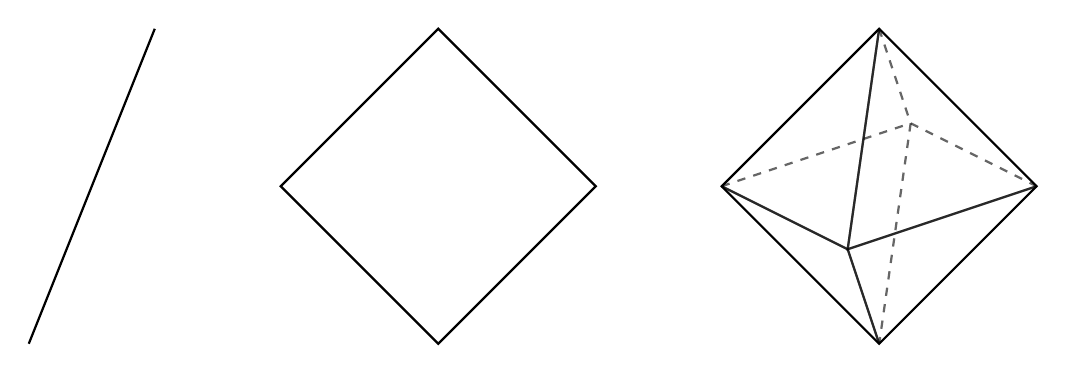
\begin{tikzpicture}[thick,scale=4]

\coordinate (D1) at (-1.8, 0.5);
\coordinate (D2) at (-2.2,-0.5);

\draw (D1) -- (D2);

\coordinate (C1) at (-1.4,0);
\coordinate (C2) at (-0.9,0.5);
\coordinate (C3) at (-0.9,-0.5);
\coordinate (C4) at (-0.4,0);

\draw (C1) -- (C2) -- (C4) -- (C3) -- cycle;

\coordinate (A1) at (0,0);
\coordinate (A2) at (0.6,0.2);
\coordinate (A3) at (1,0);
\coordinate (A4) at (0.4,-0.2);
\coordinate (B1) at (0.5,0.5);
\coordinate (B2) at (0.5,-0.5);

\begin{scope}[thick,dashed,,opacity=0.6]
\draw (A1) -- (A2) -- (A3);
\draw (B1) -- (A2) -- (B2);
\end{scope}
\draw[opacity=0.6] (A1) -- (A4) -- (B1);
\draw[opacity=0.6] (A1) -- (A4) -- (B2);
\draw[opacity=0.6] (A3) -- (A4) -- (B1);
\draw[opacity=0.6] (A3) -- (A4) -- (B2);
\draw (B1) -- (A1) -- (B2) -- (A3) --cycle;
\end{tikzpicture}
  \caption{Cross polytopes in dimensions one, two and three.}
  \label{fig:cross}
\end{figure}

\subsection{Homology Theory}
Now a very important tool in algebraic topology is introduced, namely \textbf{Homology Theory} of topological spaces. For the basic definitions from Category theory and Homological Algebra needed in the following see \cite{rotmann2009}.  

\begin{cons}
  Let $S$ be a finite set and $p \in \mathbb{P}$. Define \[A(S) := \{f \in \Z^S\colon |\im f| < \infty \}\] be maps from $S$ to $Z_p$ with finite image. $A(S)$ is an abelian group together with the operation of pointwise addition of maps.
  Then the set \[\{\mathds{1}_x\colon x\in S\} \subseteq A(S)\] forms a basis of the abelian group $A(S)$.
  Let $T$ be another set. For a map $\varphi\colon S \to T$ define the map $A(T; p)$ as
  \begin{equation*}
    A(\varphi)\colon A(S) \to A(T),\; f \mapsto \sum\limits_{x \in S}f(x)\cdot \mathds{1}_{\varphi(x)}.
  \end{equation*}
  This map is a homomorphisms of abelian groups.
\end{cons}

\begin{proof} 
  The fact that $A(S)$ is abelian follows from the fact that the group $\Z$ is abelian and thus the pointwise addition is associative and commutative, the neutral element is the constant $0$ function and the inverse of an element $f \in A(S)$ is defined as $f^{-1}(s) = -f(s)$ for $s \in S$.

  Now let $f \in A(S)$ and consider the function \[\tilde{f}\colon S \to \Z, \: s \mapsto \sum\limits_{x\in S} \alpha_x \mathds{1}_x(s)\] with $\alpha_x = f(x)$ for all $x \in S$. Let $s \in S$. It follows that
  \begin{equation*}
    \tilde{f}(s) = \sum\limits_{x \in S} \alpha_x \mathds{1}_x(s) = \alpha_s = f(s).
  \end{equation*}

  Now let $f,g \in A(S)$.
  \begin{align*}
    A(\varphi)(f+g^{-1}) &= \sum\limits_{x\in S} (f+g^{-1})(x)\cdot \mathds{1}_{\varphi(x)} \\
                        &= \sum\limits_{x\in S} (f(x)-g(x)))\cdot \mathds{1}_{\varphi(x)} \\
                        &= \sum\limits_{x\in S} f(x)\cdot\mathds{1}_{\varphi(x)} + (-g(x))\cdot \mathds{1}_{\varphi(x)} \\
                        &= \sum\limits_{x\in S} f(x)\cdot\mathds{1}_{\varphi(x)} + \sum\limits_{x\in S} (-g(x))\cdot \mathds{1}_{\varphi(x)} \\
                        &= A(\varphi)(f) + A(\varphi)(g)^{-1}.  
  \end{align*}
\end{proof}

Since the collection of indicator functions is a basis of $A(S)$ it is a convention to write elements of $A(S)$ as formal linear combinations of elements of the generating set $S$. This means the group $A(S)$ can also be represented as
\begin{equation*}
  A(S) = \left\{\sum\limits_{i=1}^k r_i x_i\colon k\in \N, \: \forall i \in \{1, \ldots, k\}\colon x_i \in S, r_i \in \Z\right\}.
\end{equation*}

\begin{thm}\label{thm:isoab}
  Let $S$ be a set and let $B$ be an abelian group. Then \[\Phi\colon \underline{\rm Ab}(A(S), B) \to B^X, \: \varphi \mapsto\varphi \circ \mathds\iota^S\footnote{$\iota^S\colon S \to A(S), \: s \mapsto \mathds{1}_s$}\] is a bijection.
\end{thm}

\begin{proof}
  The map $\Phi$ is a homomorphism in of abelian groups. To this end let $\varphi, \psi \in \underline{\rm Ab}$.
  The claim follows from the fact that $\varphi$ and $\psi$ are homomorphisms and \[(\varphi + \psi)(\mathds{1}_x) = \varphi(\mathds{1}_x) + \psi(\mathds{1}_x).\]
  Let $\varphi \in \underline{\rm Ab}(A(S), B)$ and assume that $\varphi \circ \iota^S = 0$. Then it holds that
  \begin{align*}
    \varphi(f) &= \varphi\left(\sum\limits_{x \in S}f(x) \cdot \mathds{1}_s\right) \\
    &= \sum\limits_{x \in S} f(x) \cdot \varphi(\mathds{1}_s) \\
    &= \sum\limits_{x \in S} f(x) \cdot 0 = 0
  \end{align*}
  for all $f \in A(S)$ and thus $\varphi = 0$. This means $\ker \Phi = \{0\}$.
  Now let $\psi \in B^S$. Then the map \[\xi\colon A(S) \to B, f \mapsto \sum\limits_{x \in S} f(x) \psi(x) \] is a homomorphism by
  \begin{align*}
    \xi(f + g) &= \xi\left(\sum\limits_{x \in S} (f+g)(x) \mathds{1}_x\right) \\
    &= \sum\limits_{x \in S}(f+g)\psi(x) \\
    &= \sum\limits_{x \in S} f(x)\psi(x) + \sum\limits_{x \in S}g(x)\psi(x) = \xi(f) + \xi(g).
  \end{align*}
  And now it follows that $\Phi(\xi) = (\xi \circ \iota^S)(x) = \mathds{1}_x(x) \cdot \psi(x) = \psi(x)$ for all $x \in X$ and hence $\Phi(\xi) = \psi$.
\end{proof}

The Theorem now tells us that any function from $X$ to an abelian group $B$ can be extended into a function from $A(X)$ to $B$ in a unique way. This may become clear looking at the commutative diagram in Figure \ref{fig:com1}.

\begin{figure}[h!]
  \centering
  % https://tikzcd.yichuanshen.de/#N4Igdg9gJgpgziAXAbVABwnAlgFyxMJZABgBpiBdUkANwEMAbAVxiRAA0QBfU9TXfIRQBGUsKq1GLNgCFuvEBmx4CRMuOr1mrRCACCACnYBKbhJhQA5vCKgAZgCcIAWyRkQOCEgBM1HHSwGNgALCAgAaxBqBiwwHRA4CBioKJBgmDoUxDAmBgZougAjGAYABX4VIRAHLEtgnFStaV0AHRb8fwA9Tmo4YKw7BsRiHnsnV2G-L0RRSW02NvoHNH75MZcfKaRZmLi2KAgcHAtUhiKS8uVBNhq6hs0peLaYAA8sOBw4AEI24LocYCLOjLfpcMxcIA
  \begin{tikzcd}
    X \arrow[d, "\iota^X"', hook] \arrow[rd, "\varphi"] &   \\
    A(X) \arrow[r, "\exists!\hat{\varphi}"', dashed]    & B
  \end{tikzcd}
  \caption{Commutative diagram showing the statement of Theorem \ref{thm:isoab}}\label{fig:com1}
\end{figure}

\begin{defin}
  Let $n\in\N$. The \textbf{geometric n-simplex} $\Delta_n$ is defined as
  \begin{equation*}
    \Delta_n := {\rm co}\{e_0\, \ldots, e_n\} \subseteq \R^{n+1}
  \end{equation*}
  where $e_i$ is the $i$-th canonical basis vector of $R_n$ for $i = 0,\ldots,n$. For all $i = 0, \ldots, n$ define the $i$-th face map as
  \begin{equation*}
    d_i\colon \Delta_{n-1} \to \Delta_n,\: (t_0,\ldots,t_{n-1}) \mapsto (t_0, \ldots, t_{i-1}, 0, t_i, \ldots, t_{n-1}).
  \end{equation*}
  Notice that $\im d_i \subseteq \Delta_n$. $\im d_i$ is called the $i$-th face of $\Delta_n$.
\end{defin}

\begin{defin}
  Let $X$ be a topological space and let $n\in \N$ and $p \in \mathbb{P}$. A \textbf{singular $n$-simplex} in $X$ is a continuous map $\sigma \in C(\Delta_n, X)$.
  Now the \textbf{singular $n$-chain group} of $X$ is defined as $C_n(X) := A(C(\Delta_n, X); p)$. An element $\sigma \in C_n(X)$ is called a singular $n$-chain in $X$.
  The map \[\partial_n\colon C_n(X) \to C_{n-1}(X),\: \sigma \mapsto \sum\limits_{i=0}^n(-1)^i(\sigma \circ d_i)\] is called the $n$-th boundary map for $n\in\N^+$. It is a homomorphisms of abelian groups. For $n < 1$ define $\partial_n$ as the zero map as well as all $C_n$ as trivial abelian groups.

  If $Y$ is another topological space and $f \in C(X, Y)$ then $C_n(f)\colon C_n(X) \to C_n(Y)$ defined on the generators $\sigma \in C_n(X)$ as
  \begin{equation*}
    C(f)(\sigma) = f \circ \sigma.
  \end{equation*}
  This map is a homomorphism of abelian groups.
\end{defin}

\begin{lemma}
  The composition $\partial_n \circ \partial_{n+1} = 0$ for all $n \in \N$.
\end{lemma}

\begin{proof}
  See \cite[Theorem 29.1]{MunAlTop}.
\end{proof}

The lemma above is the so called fundamental theorem of homology theory. It allows for the following definition.

\begin{defin}
  Let $X$ be a topological space, then \[C_\bullet(X) := ((C_n(X))_{n\in \Z}), (\partial_n)_{n\in \Z})\] with
  \[C_n(X) = \{0\}, \: \partial_n := 0\] for $n \in \Z\setminus\N$ is a chain complex.
\end{defin}

\begin{lemma}
  Let $X, Y$ be topological spaces and $f \in C(X, Y)$, then \[\forall n\in \N\colon \partial_n \circ C_n(f) = C_{n-1}(f) \circ \partial_n.\]
\end{lemma}

\begin{proof}
  Let $n \in \N^+$ and let $\sigma \in C(\Delta_n, X)$ then
  \begin{align*}
    \partial_n(C_n(f)(\sigma)) &= \partial_n(f\circ\sigma) \\
    &= \sum\limits_{i=0}^n(-1)^if\circ\sigma\circ d_i \\
    &= \sum\limits_{i=0}^n(-1)^iC_{n-1}(f)(\sigma\circ d_i) \\
    &= C_{n-1}(f)(\sum\limits_{i=0}^n(-1)^i(\sigma\circ d_i)) \\
    & = C_{n-1}(f)(\partial_n(\sigma)).
  \end{align*}
\end{proof}

From the previous lemma it is clear that $C_\bullet(f) := (C_n(f))_{n\in \Z}$ with $C_n(f) = 0$ for $n < 0$ is a homomorphism between chain complexes $C_\bullet(X)$ and $C_\bullet(Y)$.

\begin{lemma}\label{lem:cfunc}
  $C_\bullet\colon \underline{\rm Top} \to \underline{\rm C}(\underline{\rm Ab})$ is a functor.
\end{lemma}

\begin{proof}
  Let $X$ be a topological space and let $n \in \N$, then \[C_n(\id_X)(\sigma) = \id_X\circ \sigma = \sigma = \id_{C_n(X)}(\sigma)\]
  for all $\sigma \in C(\Delta_n, X)$ and hence $C_n(\id_X) = \id_{C_n(X)}$.
  For $n < 0$ this is trivial.

  Let $Y, Z$ be topological spaces and $f \in C(X, Y), g\in C(Y, Z)$, then for $n\in \N$ it follows that \[C_n(g\circ f)(\sigma) = g\circ f \circ \sigma = C_n(g)(f\circ \sigma) = (C_n(g) \circ C_n(f))(\sigma)\] for all $\sigma \in C(\Delta_n, X)$ and thus $C_n(g \circ f) = C_n(g) \circ C_n(f)$.
  Again the case for $n < 0$ is trivial.
\end{proof}

\begin{thm}\label{thm:hfunc}
  Let $n \in \N$. Then \[H_n\colon \underline{\rm Top} \to \underline{\rm Ab} \]
  defined by \[H_n(X) := H_n(C_\bullet(X)), \: H_n(f) := H_n(C_\bullet(f))\]
  for a topological spaces $X$ and $Y$ and $f \in \underline{\rm Top}$ is called the $n$-th singular homology group and  is a functor. 
\end{thm}

\begin{proof}
  Follows from the fact that the composition of functors is again a functor and Lemma \ref{lem:cfunc}.
\end{proof}

\begin{thm}\label{thm:hhom}
  Let $X$ and $Y$ be topological spaces. Then if $f, g\in C(X, Y)$ are homotopic maps it follows that \[H_n(f) = H_n(g)\] for all $n \in \N$.
\end{thm}

\begin{proof}
  See \cite[p. 112f]{hatcher}.
\end{proof}

\begin{col}
  Let $X$ and $Y$ be topological spaces and $f \in C(X, Y)$ is a homotopy equivalence between them, then $H_n(f)\colon H_n(X) \to H_n(Y)$ is an isomorphism for all $n \in \Z$.
\end{col}

\begin{proof}
  This follows directly from Theorem \ref{thm:hhom}.
\end{proof}

\begin{ex}
  Take a topological space $X$. Then $H_0(X) \cong \Z^n$ where $n \in \N$ is the number of path-connected components in $X$. 
\end{ex}

The example above implies that the $0$-th homology group of for example a one point space is $\Z$. This complicates some other results in homology theory. Therefore there is a version of the homology groups called \textbf{reduced} homology groups $\tilde{H_n}$ where $\tilde{H}_n(X) = H_n(X)$ for all $n \in\N^+$ and $\tilde{H}_n \oplus \mathbb{Z} = H_n(\Z)$. This means that the $0$-th reduced homology group of a one point space the trivial group is instead of $\mathbb{Z}$.
A detailed derivation of the reduced groups can be found in \cite[p. 110]{hatcher}.

\begin{defin}
  Let $G_\alpha$ be an abelian group for each $\alpha$ in an arbitrary index set $I$. Then the \textbf{external direct sum} of the groups is defined as
  \begin{equation*}
    \bigoplus\limits_{\alpha \in I}G_\alpha = \{(g_\alpha)_{\alpha\in I}\colon g_i\in G_i \: \land \: g_i \neq e_{G_i} \text{ for only finitely many indicies } i \in I\}.
  \end{equation*}
  This is again an abelian group with the operation \[(g)_{\alpha \in I} \cdot (h)_{\alpha\in I} = (g_\alpha \cdot_{G_\alpha} h_\alpha)_{\alpha \in I}.\]
  If $f_\alpha$ is a homomorphism with \[f_\alpha\colon G_\alpha \to H\]  for each $\alpha \in I$ where $H$ is an abelian group. Then
  \begin{equation*}
    \bigoplus\limits_{\alpha\in I}f_\alpha\colon \bigoplus_{\alpha \in I} G_\alpha\to H,\: (g)_{\alpha \in I} \mapsto \sum\limits_{\alpha \in I}f_\alpha(g_\alpha)
  \end{equation*}
  is a well-defined homomorphism since only finitely many summands are non-trivial.
\end{defin}

\begin{defin}
  Let $X$ be a topolgical space and let $A \subseteq X$ be a non-empty closed subspace, that is a deformation retract of a neighborhood in $X$. Then $(X, A)$ is a \textbf{good pair}.
\end{defin}

\begin{lemma}\label{lem:holwe}
  Let $X_\alpha$ be a sequence of topological spaces with basepoints $x_\alpha\in X_\alpha$ and let $\iota_\alpha\colon X_\alpha \to \bigvee\limits_{\alpha \in I}X_\alpha$ for $\alpha \in I$ where $I$ is an arbitrary index set such that $(X_\alpha, x_\alpha)$ are good. Then it holds that the maps $\iota_\alpha$ induce an isomorphism
  \begin{equation*}
    \bigoplus_{\alpha \in I}H_n(\iota_\alpha) \colon \bigoplus\limits_{\alpha\in I} \tilde{H}_n(X_\alpha)\to \tilde{H}_n\left(\bigvee\limits_{\alpha\in I} X_\alpha\right).
  \end{equation*}
\end{lemma}

\begin{proof}
  See \cite[Corollary 2.25]{hatcher}.
\end{proof}

Proofs in the later sections will only involve reasoning about homology groups. Their is a dualized concept of homology called cohomology.
The dualization in the sense of category theory works be replacing the homology groups in the chain complex by $\underline{\rm Grp}(H_n(X); G)$ where $G \in \underline{\rm Ab}$ is an abelian group. There is no need to also develop the theory of cohomology in this thesis nor a need to use it later in the proofs because of the following result. Its called \textbf{Alexander duality} and connects homology and cohomology groups.

\begin{thm}\label{thm:alex}
  Let $n \in \N$. If $A \subseteq \mathbb{S}^n$ is a compact and non-empty subspace and ($\mathbb{S}^n, A$) is triangulable\footnote{This means that $A \subseteq \mathbb{S}^n$ and that there exists a triangulation $\mathcal{K}$ of $\mathbb{S}^n$ and a subcomplex $\mathcal{K}_0 \subseteq \mathcal{K}$ with an homeomorphism $(\mathcal{K}, \mathcal{K}_0) \to (\mathbb{S}^n, A)$.} then
  \begin{equation*}
    \tilde{H}^k(A) \cong \tilde{H}_{n-k-1}(\mathbb{S}^n \setminus A)
  \end{equation*}
  for all $k \in \N$.
\end{thm}

\begin{proof}
  See \cite[Theorem 71.1]{MunAlTop}.
\end{proof}

\begin{defin}
  Let $(G_n)_{n\in\N}$ be a sequence of abelian groups and let $(\varphi_n)_{n\in\N}$ be a sequence of homomorphisms such that
  \begin{equation*}
    \varphi_n\colon G_n \to G_{n-1}
  \end{equation*}
  for $n \in \N^+$ and $\varphi_0\colon G_0 \to 0$.
  The sequence is called \textbf{exact} if
  \begin{equation*}
    \im\varphi_{n+1} = \ker\varphi_n.
  \end{equation*}
  for all $n \in \N$.
  An exact sequence of the form
  \begin{equation*}
    0 \to A \to B \to C \to 0
  \end{equation*}
  that is exact is called a \textbf{short exact sequence}.
\end{defin}

A second important tool linking homology and cohomology groups is the \textbf{universal coefficient theorem}. The next theorem is a version of it.

\begin{thm}\label{thm:uct}
Let $C_n(X)$ be a chain complex of free abelian groups and the corresponding homology groups $H_n(X)$ of $C_n(X)$ for a topological space $X$, then the cohomology groups $H^n(X; G)$ for a abelian group $G$ are determined by the exact sequence
  \begin{equation*}
    0 \to {\rm Ext}(H_{n-1}(X), G) \to H^n(X; G) \to \underline{\rm Ab}(H_n(X), G) \to 0.
  \end{equation*}
  For the definition of the ${\rm Ext}$-functor look in \cite[p. 195]{hatcher}.
\end{thm}

\begin{proof}
  See \cite[Chapter 3.1]{hatcher}.
\end{proof}

We will need only the following corollary from this theorem.

\begin{col}\label{col:hntriv}
  Let $C_n(X)$ be a chain complex of free abelian groups and $H_n(X)$ the corresponding homology groups with $H_n(X) \cong 0$ for $0 \leq n \leq k \in \N$. Then the cohomology groups are all trivial up to $k$. 
\end{col}

\subsection{Theorem of Mayer-Vietoris}
Often we can calculate the homology of simple subspaces of a larger space and want to deduce the homology of the larger space from them.
This can be accomplished with the \textbf{Mayer-Vietoris-Sequence} which is a homological version of the \textbf{Van Kampen-Theorem} (see \cite[Chapter 1.2]{hatcher}).

\begin{thm}\label{thm:mvs}
  Let $X$ be a topological space and let $A, B \subseteq X$ subspaces of $X$ such that \[X = \dot{A} \cup \dot{B}, \: A \cap B \neq \emptyset.\]
  The \textbf{Mayer-Vietoris-Sequence}
  \begin{equation*}
    \ldots \to H_n(A\cap B) \overset{\Phi}{\to} H_n(A) \oplus H_n(B) \overset{\Psi}{\to} H_n(A \cup B) \overset{\partial}{\to} H_{n-1}(A\cap B) \to \ldots \to 0
  \end{equation*}
  is an exact sequence where the mappings $\Phi$ and $\Psi$ are defined as
  \begin{align*}
    &\Phi\colon H_n(A\cap B) \to H_n(A) \oplus H_n(B),\: z + B_n(A\cap B) \mapsto (z+B_n(A), -z + B_n(B)), \\
    &\Psi\colon H_n(A) \oplus H_n(B) \to H_n(A\cup B), \: (z_1+ B_n(A), z_2 + B_n(B)) \mapsto (z_1 + z_2) + B_n(A \cup B).
  \end{align*}
\end{thm}

\begin{proof}
  For a detailed derivation of this Theorem look at \cite[p. 149]{hatcher}. 
\end{proof}

\begin{ex}
  The homology group of the $n$-dimensional sphere $\mathbb{S}^n$ are as follows
  \begin{equation*}
    H_k(\mathbb{S}^n) \cong \begin{cases}
      0, &n \neq k, \\
      \mathbb{Z}, &n = k,
    \end{cases}
  \end{equation*}
  for $k \in \Z$.
\end{ex}

\begin{proof}
  Let $A$ be the upper hemisphere and $B$ the lower hemisphere of $\mathbb{S}^n$. Then $A\cap B = \mathbb{S}^{n-1}$. Consider the Mayer-Vietoris sequence of this decomposition
  \begin{equation*}
    \ldots \overset{\partial'}{\to} H_k(\mathbb{S}^{n-1}) \to H_k(A) \oplus H_k(B) \to H_k(\mathbb{S}^n) \overset{\partial}{\to} H_{k-1}(\mathbb{S}^{n-1}) \to \ldots \to 0.
  \end{equation*}
  Since $A$ and $B$ are contractible it follows that $H_n(A) \cong H_n(B) \cong 0$ for all $n \in N$. This means that
  \begin{align*}
    0 &= \im \Psi = \ker \partial_k \\
    H_k(\mathbb{S}^{n-1}) &= \ker \Phi = \im \partial_{n+1}.
  \end{align*}
  We get that the maps $\partial\colon H_k(\mathbb{S}^n) \to H_{k-1}(\mathbb{S}^{n-1})$ are isomorphism. And thus with the fact that $H_1(\mathbb{S}^1) \cong \Z$ the claim is proven by induction on $k$.\footnote{The fact that the first homology group of $\mathbb{S}^1$ is isomorphic to $\Z$ can easily be proven with another type of homology, namely simplicial homology \cite[p. 106]{hatcher}. And since the singular and simplicial homology groups are isomorphic for triangulable spaces it can be deduced that $H_1(\mathbb{S}^1) \cong \Z$ also in the singular case. A triangulation of $\mathbb{S}^1$ is the circle graph with three vertecies.}
\end{proof}


\section{Graph Theory}
\section{$L_0$-Groups and Ameanability}

\clearpage
\bibliographystyle{alpha}
\bibliography{ref}

\end{document}
